% !TEX root = ./informe.tex

\section{Motivación}

Un \textit{clique} en un grafo $G$ es un subconjunto de vértices que induce en $G$ un subgrafo completo. La \textit{frontera} de un subconjunto de vértices $S$ es el conjunto de vértices con un extremo en $S$ y otro en $G \setminus S$. El presente informe analiza el problema de encontrar un clique que maximice la cardinalidad de su frontera en un grafo determinado. Dicho problema pertenece a la clase $NP$, por lo que es un problema dificil de resolver, y será de interés qué calidad de respuestas podemos conseguir en un tiempo razonable. \\

Antes de embarcarnos en esta aventura (lol) \todo{lol}, veamos por qué calcular el clique con máxima frontera de un grafo es un problema interesante con posibles aplicaciones reales. Primero hablaremos un poco de qué puede llegar a modelar un `clique', y que información de este puede darnos su frontera. \\

La palabra `clique' proviene de la sociologia, en donde representa un grupo unido de individuos con intereses en común. Modelando redes sociales con grafos, la definición formal de clique que acabamos de realizar hasta cierto punto coincide con esta noción. Esto ocurre porque el hecho de que un grupo de personas en una red induzca un subgrafo completo implica que todas las personas están conectadas entre sí. Esto nos da la pauta de que podríamos calcular `cliques' para conocer mejor las dinámicas dentro de una red social. También pueden utilizarse en el contexto de la química, por ejemplo, para detectar similaridades estructurales entre proteinas distintas \cite{proteins}. Pensando en el complemento de un grafo, también pueden ayudarnos a encontrar conjuntos de vértices independientes. \\

Orientados al problema CMF, el caso de las redes sociales es de particular interés. Mencionamos que un `clique' puede representar un grupo cohesivo de personas. Una observación razonable es que adyacencia total dos a dos puede ser una condicción demasiado restrictiva para caracterizar a un grupo en un modelo estándar de relaciones personales. Sin embargo, hay formas de sortear estos problemas, como utilizar la definición de \textit{n-cliques} (Luce 1950, Alba 1973), que grosso modo, es una estrategia para relajar las adyacencias dentro de un grafo. El objetivo es admitir grupos como n-cliques que no calificarian estrictamente como cliques. De cualquier forma, lo que queremos transmitir es que generalmente es posible asumir que la definición clique se corresponde bien con los grupos en redes sociales modeladas como grafos. \\

Lidiando con redes sociales con mucha información, podemos utilizar los cliques para presentar la información de forma más compacta y más representativa, lidiando con grupos en vez de individuos. \\

\vspace{-1cm}
\begin{center}
	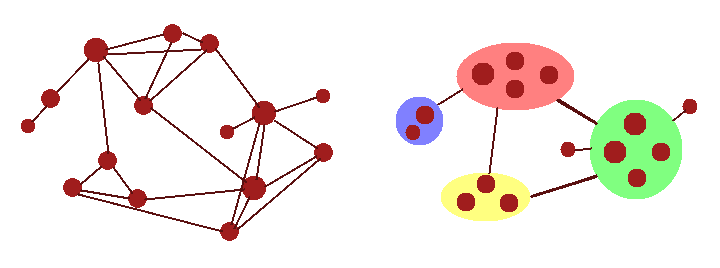
\includegraphics[scale=0.9]{informe/imgs/example.png}
	\textit{A la izquierda un grafo que modela una pequeña hipotética red social. A la derecha representamos la misma red social agrupando los individuos mediante cliques disjuntos maximales. En esta última imagen, los ejes entre cliques representan la existencia de elementos en ambos conjuntos que están conectados entre sí.}
\end{center}

Vemos como esto puede permitirnos identificar mejor las dinámicas grupales. Además, parece apropiado analizar redes sociales en torno a los grupos dentro de la misma, ya que son una unidad más representativa en términos del impacto que tienen en la red. \\

Al pensar en cliques representativos de una red, una idea sencilla es buscar los cliques más grandes, maximizando la cantidad de vértices. No es la única forma, y aquí es justamente donde entra la definición de frontera. ¿Qué representa una frontera para un clique? Por definición, son todas las conexiones que `cruzan' el clique, esto es, que conectan algún miembro del clique con alguién de afuera. Si medimos qué tan conocido es un individuo por la cantidad de amigos que tiene, entonces tiene sentido medir qué tan conocido es un clique por la cantidad de conexiones que tiene al exterior, en otras palabras, la cardinalidad de su frontera. Por lo tanto, en este caso resolver CMF representaría encontrar el grupo con más influencia dentro de una red social. \\
